% !TeX root = ..\main.tex

\section{Neo4j Features} \label{sec:features}

In this section, we discuss the features and capabilities of Neo4j, including its query language, drivers, scalability, and optimizations.

% Cypher Query Language:
Neo4j uses a query language called Cypher, which is a declarative language designed specifically for working with graph data. Cypher provides an intuitive way to express complex graph queries using patterns and traversals. In the following section \ref{subsec:Cypher}, we will explain the syntax and semantics of Cypher in detail.

% Native Drivers:
One of the key features of Neo4j is its support for native drivers in most popular programming languages. This means that developers can interact with Neo4j using their preferred language, without the need for complex APIs or libraries. Native drivers are available for Java, Python, .NET, JavaScript, and many other languages. \parencite{neo4j:mainpage}

% Cloud-Ready:
Neo4j is designed to work in cloud environments, with a focus on both vertical and horizontal scalability. It can be deployed in a variety of cloud platforms, including AWS, Microsoft Azure, and Google Cloud Platform. Neo4j's architecture is also optimized for cloud-based deployments, with features like automatic failover and backup, multi-zone replication, and load balancing. \parencite{neo4j:mainpage}

% Optimizations:
Neo4j employs a number of optimizations to efficiently handle complex graph data structures. One of these is in-memory graph processing, which allows Neo4j to store and manipulate graphs in RAM, resulting in significant performance gains. Other optimizations include caching, indexing, and compression.
% Query Performance:
Compared to traditional relational databases, Neo4j outshines in query performance by orders of magnitude. This is because graph databases are specifically designed to handle complex relationships between data points, which can be challenging to model and query using traditional relational databases. Neo4j's performance advantage is especially evident when dealing with large, interconnected datasets. \parencite{performance}

% Clustering and Replication:
To support large-scale deployments, Neo4j includes built-in support for clustering and replication. This allows Neo4j to seamlessly scale horizontally, by distributing data across multiple nodes in a cluster. Neo4j's clustering and replication features are designed to be highly available and fault-tolerant, ensuring that data is always accessible and consistent. \parencite{noe4j:clustering}

% Conclusion:
In conclusion, Neo4j is a powerful and efficient graph database that offers a number of unique features and capabilities. Its support for Cypher, native drivers, cloud deployments, optimizations, and clustering and replication make it an ideal choice for developers and organizations working with complex graph data structures.

\subsection{Cypher} \label{subsec:Cypher}

Cypher is the query language of Neo4j. It is a declarative language, which means that you describe what you want to achieve, but not how it should be done. As it is a graph query language, it is designed to work with graph data structures. On the first look it has similarities with ASCII-art.

\begin{figure}[!h]
    \centering
    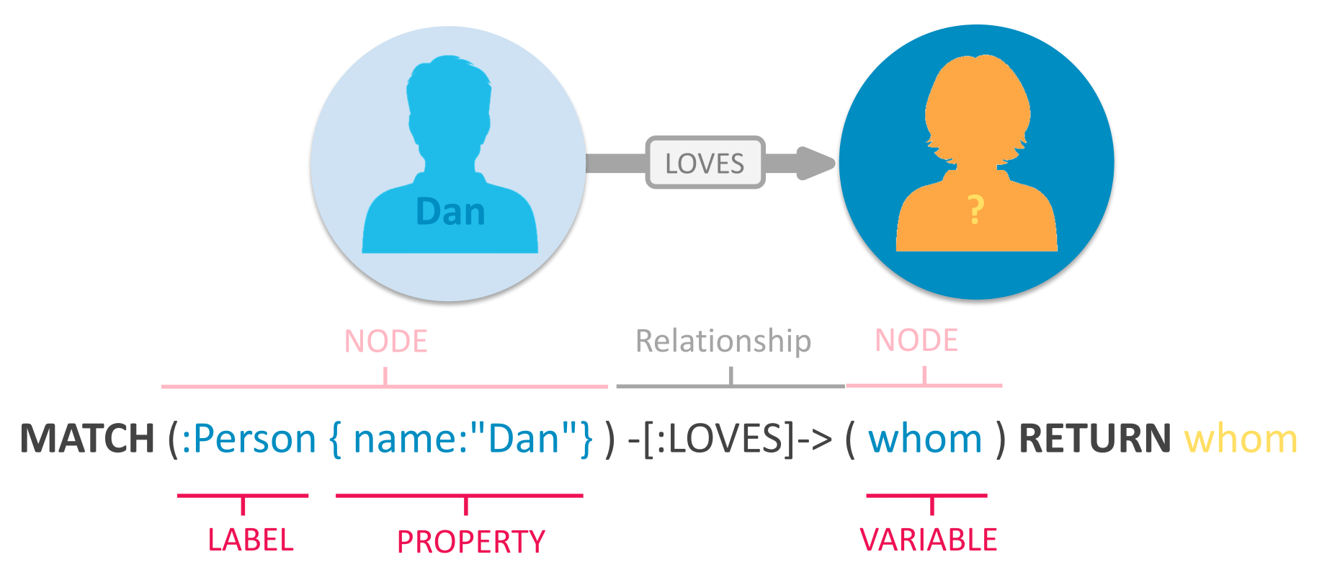
\includegraphics[width=1 \linewidth]{images/cypher_example.png}
    \caption{Cypher Query Language Basics \parencite{neo4j:cypher}} \label{img:cypher}
\end{figure}

In the example in Figure \ref{img:cypher} you can see the basic structure of a Cypher query. It starts with a “MATCH” statement, which is used to find the nodes and relationships you want to work with. Nodes are represented by round brackets and relationships by square brackets with ASCII-art like arrows to show the direction of the relationship. Inside those brackets you can specify the labels of the nodes and the type of the relationship. Additional properties can be specified with curly brackets. In this example the second node in the query has a variable name, which is used to refer to it in the following statements. After the “MATCH” statement you can specify the “RETURN” statement, which is used to return the results of the query. In this example the “RETURN” statement returns the variable name of the second node.

